\documentclass[11pt, a4paper]{article}
\usepackage[english]{babel}
\usepackage[utf8]{inputenc}
\usepackage{fancyhdr}
\usepackage{lastpage}
\usepackage{datetime}
\usepackage{indentfirst}
\usepackage{hyperref}
\usepackage{appendix}
\usepackage{amsmath}
\usepackage{amssymb}
\usepackage{amsfonts}
\usepackage{mathtools}
\usepackage{siunitx}
\usepackage{cancel}
\usepackage{tabularray}
\usepackage{multirow}
\usepackage{array}
\usepackage{hhline}
\usepackage{makecell}
\usepackage{courier}
\usepackage[font=small, skip=0pt]{caption}
\usepackage[font=scriptsize, skip=0pt]{subcaption}
\usepackage{float}
\usepackage{graphicx}
\usepackage{listings}
\usepackage{xcolor}
\usepackage{matlab-prettifier}
\usepackage[T1]{fontenc}
\usepackage{lmodern}
\usepackage{bigfoot}
\usepackage{filecontents}
\usepackage[nottoc]{tocbibind}

\graphicspath{ {./mathimages/} }

\newdateformat{Datea}{\THEDAY\ \monthname[\THEMONTH] \THEYEAR}
\newdateformat{Dateb}{\monthname[\THEMONTH] \THEYEAR}

%\allowdisplaybreaks
\DeclareMathOperator{\cosec}{cosec}
\DeclareMathOperator{\cotan}{cotan}
\DeclareMathOperator{\sech}{sech}
\DeclareMathOperator{\cosech}{cosech}
\DeclareMathOperator{\arcsec}{arcsec}
\DeclareMathOperator{\arccot}{arccot}
\DeclareMathOperator{\arccsc}{arccosec}
\DeclareMathOperator{\arccosh}{arccosh}
\DeclareMathOperator{\arcsinh}{arcsinh}
\DeclareMathOperator{\arctanh}{arctanh}
\DeclareMathOperator{\arcsech}{arcsech}
\DeclareMathOperator{\arccsch}{arccsch}
\DeclareMathOperator{\arccoth}{arccoth}
\DeclareMathOperator{\arsinh}{arsinh}
\DeclareMathOperator{\arcosh}{arcosh}
\DeclareMathOperator{\artanh}{artanh}

\DeclareMathOperator{\cis}{cis}

\pagestyle{fancy}
\fancyhf{}
\rhead{Hatam Barma}
\chead{\begin{tabular}[t]{@{}l@{}}\\Mathematics and Further Mathematics Pure Revision Summary\end{tabular}}
\lhead{\Dateb\today}
\cfoot{Page \thepage}

\renewcommand{\thesection}{\arabic{section}} 

\renewcommand{\thesubsection}{\thesection.\arabic{subsection}}

\setcounter{section}{1}

\allowdisplaybreaks

\fancypagestyle{plain}{
\fancyhf{}
\renewcommand{\headrulewidth}{0pt}}

\hypersetup{
    colorlinks,
    citecolor=black,
    filecolor=black,
    linkcolor=blue,
    urlcolor=magenta!70!black
}

\begin{document}


\begin{titlepage}
   \begin{center}
       \vspace*{2.5cm}
	\huge
       \textbf{A-Level Mathematics and Further Mathematics Pure Revision Summary} \\
	\vspace{1cm}
	\Large
       \textbf{Chapter 2: Calculus I: Differentiation}
            
       \vspace{1.5cm}
	\LARGE
       \textbf{Hatam Barma} \\
	\vspace{0.75cm}
       \normalsize
       \emph{Compiled on \Datea\today} \\

       \vfill
        

	E-mail: hatam.barma@gmail.com
   \end{center}
\end{titlepage}


\tableofcontents

\clearpage
\section{Calculus I: Differentiation}
\vspace{0.5cm}

\subsection{Differentiation and derivatives -- Tangent and normal}
\begin{itemize}
\item A Level M AS / Year 1 \hspace{1cm} \phantom{ } Pages 251 -- 260 
\item A Level M AS / Year 1 \hspace{1cm} \phantom{ } Pages 271 -- 274
\end{itemize} \par
Differentiation of a function gives the instantaneous rate of change (tangent) to that function. 
From first principles, differentiation is defined as:
\begin{equation*}
f'(x)=\lim_{h \to 0}\left[ \frac{f(x+h)-f(x)}{h} \right]
\end{equation*}
This is explicitly the formula for the gradient of the chord $PQ$, where $P$ and $Q$ have coordinates $(x,f(x))$ and $(x+h,f(x+h))$ respectively, in the limit where $h$ tends to zero. \newline \par
Learning how to differentiate combinations of functions is also necessary. Intuitively, we can see that a simple addition (or subtraction) of functions $h(x)=f(x)\pm g(x)$ has a derivative $h'(x)=f'(x)\pm g'(x)$ by putting $h(x)$ into the definition above. Sections \ref{chainrule}, \ref{productrule}, and \ref{quotientrule} show how to differentiate pairs of functions combined in different ways. \newline \par
The derivative of a function at a point gives the gradient of the tangent at that point. The straight-line equation of the tangent to a point $(a,b)$ is given by
\begin{equation*}
y-b=m(x-a)
\end{equation*}
where $x$ and $y$ are general points in space, $a$ and $b$ are the coordinates of the specific point, and $m$ is the gradient of the tangent (value of the derivative). If we wish to find the equation of the straight-line normal to the point, that has a gradient equal to the negative reciprocal of the gradient of the tangent. \newline \par
Derivatives of a function $y=y(x)$ can be denoted by $\frac{\mathrm{d}y}{\mathrm{d}x}$ (Leibniz notation) or $y'(x)$ (Lagrange notation). Higher derivatives are expressed as $\frac{\mathrm{d}^{n}y}{\mathrm{d}x^{n}}$ (Leibniz) or $y^{(n)}(x)$ (Lagrange). For smaller values of $n$, Lagrange notation makes use of repeated primes ($'$), i.e. $y''(x)$, $y''(x)$, etc. but for higher $n$, this becomes unwieldy. \newline \par

Newton also introduced `dot-notation' for time derivatives. Conventionally, this is only used when dealing with functions of times, so for the function $x=x(t)$, $\dot{x}=\frac{\mathrm{d}x}{\mathrm{d}t}$, $\ddot{x}=\frac{\mathrm{d}^{2}x}{\mathrm{d}t^{2}}$, etc.
\vspace{0.5cm}


\subsection{Useful derivatives to know}
\label{usefulderivatives}
Here is a list of derivatives of simple functions. They can of course be manipulated in the usual way using the chain rule (section \ref{chainrule}), product rule (section \ref{productrule}), and quotient rule (section \ref{quotientrule}). 

\begin{figure}[H]
\centering
\begin{subfigure}[b]{0.49\textwidth}
\centering
\begin{tblr}{|[.75pt]|c|c||[.75pt]}
\hline[1.25pt]
\textbf{$f(x)$} & \textbf{$f'(x)$}  \\ \hline[0.75pt]
constant & 0 \\ \hline
$x^{n}$ & $nx^{n-1}$ \\ \hline
$e^{x}$ \small{\emph{or}} $\exp(x)$ &  $e^{x}$ \small{\emph{or}} $\exp(x)$ \\ \hline
$\ln(x)$ & $\frac{1}{x}$ \\ \hline
$\sin(x)$ & $\cos(x)$  \\ \hline
$\cos(x)$ & $-\sin(x)$  \\ \hline
$\tan(x)$ & $\sec^{2}(x)$  \\ \hline
$\sec(x)$ & $\sec(x)\tan(x)$  \\
\hline[.75pt]
\end{tblr}
\end{subfigure}
\hfill
\begin{subfigure}[b]{0.49\textwidth}
\centering
\begin{tblr}{|[.75pt]|c|c||[.75pt]}
\hline[1.25pt]
\large{\textbf{$f(x)$}} & \large{\textbf{$f'(x)$}}  \\ \hline[0.75pt]
$\cosec(x)$ & $-\cosec(x)\cotan(x)$  \\ \hline
$\cotan(x)$ & $-\cosec^{2}(x)$ \\ \hline
$\sinh(x)$ &  $\cosh(x)$ \\ \hline
$\cosh(x)$ & $\sinh(x)$ \\ \hline
$\tanh(x)$ & $\sech^{2}(x)$  \\ \hline
$\sech(x)$ & $-\sech(x)\tanh(x)$  \\ \hline
$\cosech(x)$ & $-\cosech(x)\coth(x)$  \\ \hline
$\coth(x)$ & $-\cosech^{2}(x)$  \\
\hline[.75pt]
\end{tblr}
\end{subfigure}
\end{figure}
\vspace{0.2cm}


\subsection{Finding stationary points and curve sketching}
\begin{itemize}
\item A Level M AS / Year 1 \hspace{1cm} \phantom{ } Pages 275 -- 279
\end{itemize} \par
Roots of an equation give $x$ intercepts; constant term (of a polynomial) gives the $y$ intercept. A single root is a basic cut, a double root is a local maximum or minimum, and a triple root is a stationary point of inflection. \newline \par 

Any stationary points are characterised by the first derivative being $0$.
\vspace{0.2cm}


\subsection{Classification of stationary points}
\begin{itemize}
\item A Level M Year 2 \hspace{1cm} \phantom{ AS / } Pages 247 -- 253
\item A Level M Year 2 \hspace{1cm} \phantom{ AS / } Pages 261 -- 267
\end{itemize} \par
The second derivative gives the gradient of the gradient of the function. Stationary points of a function $f(x)$ can be classified as follows:
\begin{equation*}
\mathrm{If\;} f'(a)=0 
\begin{cases}
f''(a)>0, & \mathrm{then\;} x=a\; \mathrm{is\; a\; minimum} \\
f''(a)<0, & \mathrm{then\;} x=a\; \mathrm{is\; a\; maximum} \\
f''(a)=0, & \text{then further investigation required}
\end{cases}
\end{equation*}
A point of inflection is a point where the second derivative changes sign $(+/-)$
\vspace{0.5cm}


\subsection{Curvature: convex, concave and point of inflection}
\begin{itemize}
\item A Level M Year 2 \hspace{1cm} \phantom{ AS / } Pages 247 -- 253
\end{itemize} \par
\begin{itemize}
\item[-] A function $f$ is said to be \underline{\textbf{convex}} over an interval $[a,b]$ if \\$f''(x)\geq0, \forall x \in[a,b]$
\item[-] A function $f$ is said to be \underline{\textbf{concave}} over an interval $[a,b]$ if \\$f''(x)\leq0, \forall x \in[a,b]$
\item[-] A \underline{\textbf{point of inflection}} on a curve $y=f(x)$ is a point where \\$f''(a)=0$ \emph{and} $f''(a)$ changes sign
\end{itemize}
\vspace{0.5cm}


\subsection{Optimisation}
\begin{itemize}
\item A Level M AS / Year 1 \hspace{1cm} \phantom{ } Pages 279 -- 287
\end{itemize} \par
Use first and second derivatives to find maximum or minimum values subject to sets of constraints
\vspace{0.5cm}


\subsection{The Chain Rule}
\label{chainrule}
\begin{itemize}
\item A Level M Year 2 \hspace{1cm} \phantom{ AS / } Pages 198 -- 202
\end{itemize} \par
The chain rule is used to differentiate \emph{composite functions} (functions of functions). It works as follows:
\begin{equation*}
\frac{\mathrm{d}}{\mathrm{d}x}\left[ f(g(x)) \right]=f'(g(x))\times g'(x)
\end{equation*}
A couple of examples:
\begin{align*}
\frac{\mathrm{d}}{\mathrm{d}x}\left[\sqrt{\text{something}}\right]&=\frac{1}{2\sqrt{\text{something}}}\times\frac{\mathrm{d}}{\mathrm{d}x}\left[\text{something}\right] \\
\frac{\mathrm{d}}{\mathrm{d}x}\left[\frac{1}{\text{something}}\right]&=-\frac{1}{\text{something}^{2}}\times\frac{\mathrm{d}}{\mathrm{d}x}\left[\text{something}\right] \\
\end{align*}
\begin{itemize}
\item[Note:] The chain rule must also be considered and applied when anti-differenti\-ating
\end{itemize}
\vspace{0.5cm}
\newpage

\subsection{The Product Rule}
\label{productrule}
\begin{itemize}
\item A Level M Year 2 \hspace{1cm} \phantom{ AS / } Pages 203 -- 205
\end{itemize} \par
The product rule is used to differentiate the \emph{product} of two functions. Here is a short derivation as to where it comes from.
\begin{figure}[H]
\centering
\begin{subfigure}[b]{0.49\textwidth}
\centering
\scalebox{.85}{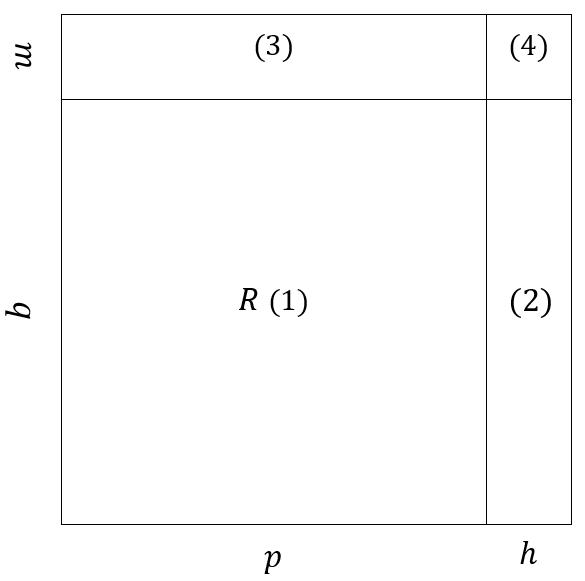
\includegraphics[width=\textwidth]{productrule1}}
\end{subfigure}
\hfill
\begin{subfigure}[b]{0.49\textwidth}
\small
First consider how the area $R$ changes when $p\rightarrow p+h$, and $q\rightarrow q+m$.
\begin{flalign*}
R&=p\cdot q, & R'=p'\cdot q' && \\
&&&&\\
R'&=(p+h)(q+m)& && \\
&=pq+hq+pm+hm & &&
\end{flalign*}
where $pq$, $hq$, $pm$, $hm$ are labelled $(1)$, $(2)$, $(3)$, and $(4)$ respectively. \\
\normalsize
\end{subfigure}
\end{figure}

\begin{figure}[H]
\centering
\begin{subfigure}[b]{0.49\textwidth}
\centering
\scalebox{.85}{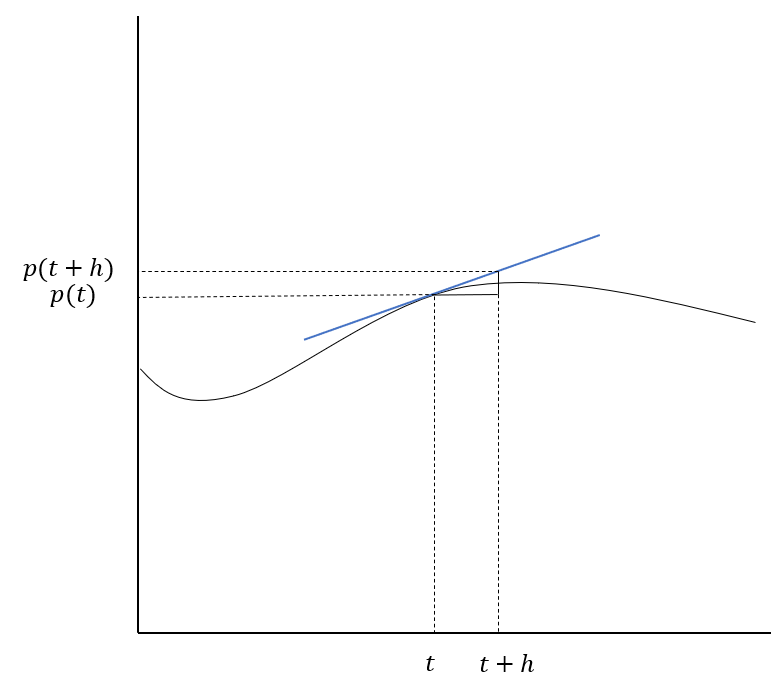
\includegraphics[width=\textwidth]{productrule3}}
\end{subfigure}
\hfill
\begin{subfigure}[b]{0.49\textwidth}
\small
Zooming in on the triangle created by the points $(t,p(t)), (t+h, p(t)), (t+h, p(t+h))$, we can approximate the distance from $p(t+h)$ to $p(t)$ by reversing our first principle form of a derivative, to give:
\normalsize
\begin{center}
\scalebox{.5}{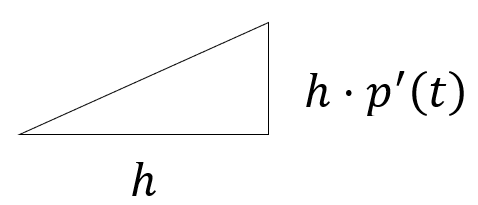
\includegraphics[width=\textwidth]{productrule2}}
\end{center}
So, we have: $p(t+h)\approx p(t)+h\times p'(t)$ \scriptsize{\emph{good if $h\rightarrow 0$}}
\normalsize
\end{subfigure}
\end{figure}
\vspace{-0.5cm}
Define $R(t)=p(t)\cdot q(t)$
\begin{flalign*}
R(t)&=p(t)\cdot q(t) && \\
R(t+h)&=p(t+h)\cdot q(t+h) && \\
R(t+h)&\approx (p(t)+h\times p'(t))\cdot (q(t)+h\times q'(t)) && \\
R(t+h)&\approx p(t)q(t)+h\left[ p'(t)q(t) + p(t)q'(t)  \right]+h^{2}\left[ p'(t)q'(t) \right] && \\
\end{flalign*}
This definition of $R(t+h)$ can then be used in the definition of the derivative from first principles;
\scriptsize
\begin{flalign*}
\frac{\mathrm{d}R}{\mathrm{d}t}&= \lim_{h \to 0} \left[ \frac{R(t+h)-R(t)}{h} \right] && \\
&= \lim_{h \to 0} \left[ \frac{\left( \cancel{p(t)q(t)}+h\left[ p'(t)q(t) + p(t)q'(t)  \right]+h^{2}\left[ p'(t)q'(t) \right] \right)-\cancel{p(t)q(t)}}{h} \right] && \\
&= \lim_{h \to 0} \left[ \frac{\cancel{h}\left[ p'(t)q(t) + p(t)q'(t)  \right]+h^{\cancel{2}}\left[ p'(t)q'(t) \right]}{\cancel{h}} \right] && \\
&=p'(t)q(t)+p(t)q'(t)+\cancel{\lim_{h\to0}\left[ h\left[p'(t)q'(t)\right] \right]} \\
\frac{\mathrm{d}R}{\mathrm{d}t}&=  p'(t)q(t) + p(t)q'(t) &&
\end{flalign*}
\normalsize
So we recover the \emph{Product Rule}
\begin{equation*}
\frac{\mathrm{d}}{\mathrm{d}x}\left[ f(x)g(x) \right] = f'(x)g(x)+f(x)g'(x)
\end{equation*}
%\vspace{0.5cm}


\subsection{The Quotient Rule}
\label{quotientrule}
\begin{itemize}
\item A Level M Year 2 \hspace{1cm} \phantom{ AS / } Pages 206 -- 209
\end{itemize} \par
The quotient rule is used to differentiate the \emph{quotient} of two functions. While a quotient is still a product, the product rule reduces to a simpler form in the case of a quotient, and so it is given a separate name. The derivation relies on the results of the chain rule and product rule (sections \ref{chainrule} and \ref{productrule} respectively).

\small
\begin{flalign*}
\frac{f(x)}{g(x)} &= f(x)g(x)^{-1} \hspace{2.75cm} \frac{\mathrm{d}}{\mathrm{d}x}\left[ g(x)^{-1} \right]=-[g(x)]^{2}\times g'(x) && \\
\frac{\mathrm{d}}{\mathrm{d}x} \left[ \frac{f(x)}{(g(x)} \right] &= \frac{\mathrm{d}}{\mathrm{d}x}\left[ f(x)\left[ g(x) \right]^{-1} \right] && \\
&=f'(x)\left[ g(x) \right]^{-1} + \left[ - \left[ g(x) \right]^{-2} \times g'(x) \right]\times f(x) && \\
&=\frac{f'(x)}{\left[ g(x) \right]} - \frac{f(x)g'(x)}{\left[ g(x) \right]^{2}} && \\
&=\frac{f'(x)g(x)}{\left[ g(x) \right]^{2}} - \frac{f(x)g'(x)}{\left[ g(x) \right]^{2}} && \\
&=\frac{f'(x)g(x)-f(x)g'(x)}{\left[ g(x) \right]^{2}} && \\
\end{flalign*}
\normalsize

Therefore, the \emph{Quotient Rule} is:
\begin{equation*}
=\frac{f'(x)g(x)-f(x)g'(x)}{\left[ g(x) \right]^{2}}
\end{equation*}
\vspace{0.1cm}

\newpage
\subsection{Implicit differentiation}
\label{implicitdifferentiation}
\begin{itemize}
\item A Level M Year 2 \hspace{1cm} \phantom{ AS / } Pages 209 -- 214
\end{itemize} \par
Implicit differentiation works in the same way as the chain rule, with the correction factor of a $y$ term being $\frac{\mathrm{d}y}{\mathrm{d}x}$. This is best illustrated by an example:
\begin{flalign*}
\frac{\mathrm{d}}{\mathrm{d}x}\left[ \left(x^{2}+4\right)^{3}\right]&=3\left( x^{2}+4\right)^{2}\times 2x && \\
&=6x\left(x^{2}+4\right)^{2} && \\
\frac{\mathrm{d}y}{\mathrm{d}x}\left[ \left( f(x)\right)^{3}\right]&=3\left( f(x) \right)^{2}\times\frac{\mathrm{d}}{\mathrm{d}x}\left[ f(x) \right] &&\\
\frac{\mathrm{d}y}{\mathrm{d}x}\left[ y^{3}\right]&=3y^{2}\times\frac{\mathrm{d}y}{\mathrm{d}x}&&
\end{flalign*} \par
\vspace{0.5cm}

\subsection{Differentiating inverse functions}
\begin{itemize}
\item A Level M Year 2 \hspace{1cm} \phantom{ AS / } Pages 214 -- 216
\end{itemize} \par
$f(x)=y$, so $x=f^{-1}(y)$ Therefore $f'(x)=\frac{\mathrm{d}y}{\mathrm{d}x}$, and by extension, the derivative of the inverse function is equal to $\frac{\mathrm{d}x}{\mathrm{d}y}=\frac{1}{\left(\frac{\mathrm{d}y}{\mathrm{d}x}\right)}$. \newline \par

This method can be used to find the derivative of inverse functions, and extends to functions such as $\arcsin, \arcosh, \ln, \text{\emph{etc.}}$. For example, take the function $y=\ln(x)$:
\begin{flalign*}
x&=e^{y} \hspace{2.75cm} y=\ln(x) && \\
\frac{\mathrm{d}y}{\mathrm{d}x}&=e^{y} && \\
\frac{\mathrm{d}y}{\mathrm{d}x}&= \frac{1}{\left(\frac{\mathrm{d}x}{\mathrm{d}y}\right)} =e^{-y} =e^{-\ln(x)}=x^{-1} =\frac{1}{x} &&
\end{flalign*}
\vspace{0.2cm}


\subsection{Parametric differentiation}
\label{parametricdifferentiation}
\begin{itemize}
\item A Level M Year 2 \hspace{1cm} \phantom{ AS / } Pages 258 -- 263
\end{itemize} \par
Parametric equations are defined in terms of an external variable, for example:
\begin{gather*}
x=f(t)\\y=g(t)
\end{gather*}
Therefore, $\frac{\mathrm{d}x}{\mathrm{d}t}=f'(t)$ and $\frac{\mathrm{d}y}{\mathrm{d}t}=g'(t)$, so:
\begin{equation*}
\frac{\mathrm{d}y}{\mathrm{d}x}=\frac{\left( \frac{\mathrm{d}y}{\mathrm{d}t} \right)}{\left( \frac{\mathrm{d}x}{\mathrm{d}t} \right)}=\frac{g'(t)}{f'(t)}
\end{equation*}
\begin{itemize}
\item[Note:] See section \ref{relatedratesofchange} for more on why we can `cancel' the $dt$ terms as with fractions
\end{itemize}
\vspace{0.5cm}


\subsection{Sketching curves}
\begin{itemize}
\item A Level M AS / Year 1 \hspace{1cm} \phantom{ } Pages 55 -- 68
\end{itemize} \par
When sketching curves, think about:
\begin{itemize}
\item[-] Intersections
\vspace{-0.25cm}
\item[-] Intercepts on axes
\vspace{-0.25cm}
\item[-] Which curves are above / below other curves (and where crossovers occur)
\vspace{-0.25cm}
\item[-] Derivatives $\rightarrow$ stationary points
\vspace{-0.25cm}
\item[-] Behaviour for large positive and negative $x$
\vspace{-0.25cm}
\item[-] Asymptotes (vertical, horizontal, oblique)
\end{itemize}
\vspace{0.5cm}


\subsection{Rational functions; polynomial curve sketching}
\begin{itemize}
\item A Level M AS / Year 1 \hspace{1cm} \phantom{ } Pages 55 -- 68
\end{itemize} \par
A rational function is defined as any function which can be expressed as a rational fraction of polynomials. \newline \par

When sketching, take out a factor of the denominator from the numerator to give the horizontal / oblique asymptote. \newline \par

For example:
\begin{flalign*}
y&=\frac{-x^{3}+5x}{x^{2}-4} && \\
&=\frac{-x\left( x^{2}-4\right)+x}{x^{2}-4} && \\
&=-x+\frac{x}{(x+2)(x-2)} \hspace{1cm} (*)
\end{flalign*}
This implies the oblique asymptote is $y=-x$, as $\lim_{x\rightarrow\pm\infty}\left[ \frac{x}{(x+2)(x-2)} \right]=0$, so for large positive and negative $x$, $y$ tends to $-x$. It is trivial to see $x=2$ and $x=-2$ are vertical asymptotes, as they are roots of the expression in the denominator, and dividing by zero is undefined. \newline \par

Lastly, we need to consider whether the curve approaches the horizontal / oblique asymptote from above or below, and whether the vertical asymptotes have the function going to positive or negative infinity. To do this, consider the parity of the numerator and denominator as $x$ approaches the vertical asymptote limits from above and below. So, in the case of $y=\frac{-x^{3}+5x}{x^{2}-4}$:

\scriptsize
\begin{center}
\begin{tblr}{|[.75pt]|c||c|c||[.75pt]}
\hline[1.25pt]
$x$ & $-2^{-}$ & $-2^{+}$ \\ \hline[.75pt]
Numerator & $-(-2^{-})^{3}+5(-2^{-})=-2^{-}<0$ & $-(-2^{+})^{3}+5(-2^{+})=-2^{+}<0$ \\ \hline
Denominator & $(-2^{-})^{2}-4=0^{+}>0$ & $(-2^{+})^{2}-4=0^{-}<0$ \\ \hline
Asymptote & $y=\frac{-2^{-}}{0^{+}}=-\infty$ & $y=\frac{-2^{+}}{0^{-}}=+\infty$ \\ 
\hline[.75pt]
\end{tblr}
\end{center}
\normalsize

\scriptsize
\begin{center}
\begin{tblr}{|[.75pt]|c||c|c||[.75pt]}
\hline[1.25pt]
$x$ &  $2^{-}$ & $2^{+}$ \\ \hline[.75pt]
Numerator & $-(2^{-})^{3}+5(2^{-})=2^{-}>0$ & $-(2^{+})^{3}+5(2^{+})=2^{+}>0$ \\ \hline
Denominator & $(2^{-})^{2}-4=0^{-}<0$ & $(2^{+})^{2}-4=0^{+}>0$ \\ \hline
Asymptote & $y=\frac{2^{-}}{0^{-}}=-\infty$ & $y=\frac{2^{+}}{0^{+}}=+\infty$ \\ 
\hline[.75pt]
\end{tblr}
\end{center}
\normalsize

We can then see from $(*)$, considering `remainder' of the asymptote, the denominator tends to $0^{+}$ as $x$ tends to $\pm\infty$. So, the parity of the `remainder' is determined by the parity of the numerator in this case, which is simply $x$. So, for $x\rightarrow+\infty$, the remainder is positive, and for $x\rightarrow-\infty$, the remainder is negative. Thus the curve approaches the asymptote from above for $x\rightarrow+\infty$ and from below for $x\rightarrow-\infty$. \newline \par

To see what all of this looks like, the figure below has the curve in red, with the asymptotes marked on in dashed lines:

\begin{figure}[H]
\centering
\begin{subfigure}[b]{0.89\textwidth}
\centering
\scalebox{0.85}{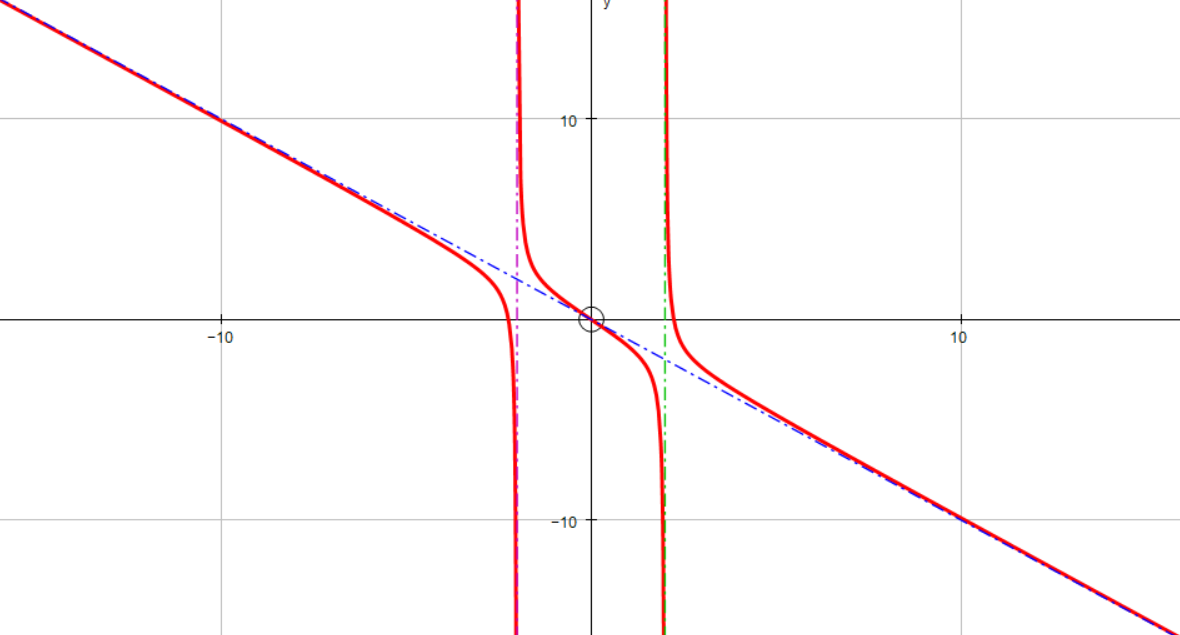
\includegraphics[width=\textwidth]{curvesketching}}
\end{subfigure}
\end{figure}

\vspace{0.5cm}

\end{document}